%%%%%%%%%%%%%%%%%%%%%%%%%%%%%%%%%%%%%%%%%%%%%%%%%%%%%%%%%%%%%%%%%%%%%%
% Fichero: PrincipalTFG.tex
% Autor: Rubén Márquez Villalta
% Fecha (creación): Febrero 2020 
% Descripción: Documento principal de la memoria del TFG
% Universidad: Escuela Superior de Informática, UCLM(Ciudad Real)
% Titulo: “Global-Manager: Entrenando mediante un Juego Serio a los 
% Jefes de Proyecto en los Desafíos del Desarrollo Global del Software”
%
% ##### Compilación #####
%
% Este documento ha sido desarrollado para compilarse con `pdflatex`,
% `biblatex` (bibliografía con `biber`).
%
% Para su compilación se aconseja utilizar `latexmk` (requiere para su 
% ejecución de un intérprete [`Perl`](http://strawberryperl.com/)):
%
% <\$> latexmk -pdf -silent -synctex=1 --enable-write18 
%
%%%%%%%%%%%%%%%%%%%%%%%%%%%%%%%%%%%%%%%%%%%%%%%%%%%%%%%%%%%%%%%%%%%%%%

% --------------------------------------------------------------------
%
% PREÁMBULO DEL DOCUMENTO TFG
%
% --------------------------------------------------------------------

% ----- Clase del documento (book) -----
\documentclass[
	11pt,			% Tamaño de letra
	a4paper,		% Tamaño de papel
	twoside,		% Impresión a doble cara
	openright,		% Apertura del capítulo a la derecha
	final			% Versión final
]{book}


% ----- Importación de paquetes -----
\usepackage[utf8]{inputenx}			% Codificación de entrada: utf8
\usepackage[english,spanish,es-tabla]{babel}	% Idioma del documento

% ## Geometría de las páginas del documento
\usepackage[		% Márgenes del documento
	top=2.5cm,		% Margen superior
	bottom=2.5cm,	% Margen inferior
	inner=3.5cm,	% Margen al interior
	outer=2cm		% Margen al exterior
]{geometry}

% ## Tipografía
\usepackage[tt=false]{libertine} 	% Libertine con Old-Style Figures
\usepackage[libertine]{newtxmath}	% Times

\usepackage[T1]{fontenc}	% Codificación de salida
\usepackage{microtype}		% Mejoras de mircrotipografía en la obtención del PDF

% ## Graficos y tablas
\usepackage{graphicx}			% Inclusión de figuras
\graphicspath{{../figuras/}}	% Path de búsqueda de ficheros gráficos
\DeclareGraphicsExtensions{.pdf,.png,.jpg,.jpeg}	% Precedencia de extensiones
\usepackage{tabularx,booktabs}

% ## Personalización de títulos de figuras y tablas
\usepackage[		% Personalización de títulos de figuras y tablas
	margin=10pt,	% Margen
	font=small,		% Tamaño de tipografía
	labelfont=bf,	% Prefijo-Etiqueta en negrita
	format=hang		% Sangrado del texto de pie de foto
]{caption}
\captionsetup[table]{skip=4pt}	% Separación del caption en las tablas

% ## Bibliografía: Biblatex con biber
\usepackage[			% Estilo de la bibliografía	
	backend=biber, 		% Backend
	sortcites,			% Citas acortadas
	defernumbers=true, 	% Para numerar al final
	style=numeric-comp, % Estilo numérico condensado
	autolang=other, 	% Requerido para opción multilingüe
	language=auto   	% Requerido para opción multilingüe
]{biblatex}
\addbibresource{biblioTFG.bib} 	% Fichero de bibliografía.

% ## Paquete de estilo para el TFG (ESI-UCLM)
\usepackage[spanish]{{../estilo/uclmTFGesi}}	% Opción de idioma de la memoria y prefijos de género.

% ## Datos del documento
\tituloPrimera{GLOBAL-MANAGER: Entrenando mediante un Juego Serio a los Jefes de Proyecto en los Desafíos del Desarrollo Global del Software}		% Título principal
\titulo{GLOBAL-MANAGER}								% Título corto
\autor{Rubén Márquez Villalta}						% Autor
\email{Ruben.Marquez@alu.uclm.es}					% E-mail del autor
\tutor{Francisco Pascual Romero Chicharro} 			% Tutor
\cotutor{Aurora Vizcaíno Barceló}					% Co-autora
\instEdu{UNIVERSIDAD DE CASTILLA-LA MANCHA}			% Universidad
\escudo{escudoInf}									% Escudo Informática
\centroEdu{ESCUELA SUPERIOR DE INFORMÁTICA}			% Centro educativo
\deptoEduPrimera{Departamento de Tecnologías y Sistemas de la Información}	% Departamento
\titulacion{GRADO EN INGENIERÍA INFORMÁTICA}		% Titulación
\especialidad{TECNOLOGÍA ESPECÍFICA DE COMPUTACIÓN}	% Tecnología especialidad
\tipoDoc{TRABAJO FIN DE GRADO}						% Tipo de documento
\fechaDef{julio, 2020} 								% Fecha de defensa
\mesDef{julio}        								% Mes de defensa
\yearDef{2020}        								% Año de defensa
\lugarDef{Ciudad Real}								% Lugar de defensa

% ## Propiedades del documento PDF
\hypersetup{
	pdftitle={Global-Manager TFG}, 		% Título
	pdfauthor={Rubén Márquez Villalta}, % Autor
	pdfsubject={TFG},  					% Tema
	pdftoolbar=true, 					% Muestra la toolbar de Acrobat
	pdfmenubar=true	 					% Muestra la menubar de Acrobat
}

% --------------------------------------------------------------------
%
% CUERPO DEL DOCUMENTO
%
% --------------------------------------------------------------------

\begin{document}
\frontmatter	% Cambio de numeración de páginas a números romanos

\pagestyle{empty}


% ---------------------------------
%
% PORTADAS
%
% ---------------------------------

\portadaTFG		% Portada principal

\portadillaTFG	% Portada interior con tutor y co-tutora


% ---------------------------------
%
% CRÉDITOS
%
% ---------------------------------

% ---------------------------------
%
% CRÉDITOS
%
% ---------------------------------

% TODO: Rellenar la página de créditos con el tipo de licencia de distribución para este TFG

\tribunalTFG	% Página para calificaciones del tribunal

% TODO: Rellenar la dedicatoria
\dedicado{Dedicatoria...}


% ---------------------------------
%
% RESUMEN
%
% ---------------------------------

% ---------------------------------
%
% RESUMEN
%
% ---------------------------------

\pagestyle{plain}	% Página con numeración inferior al pie


% ----- Resumen del documento -----
\selectlanguage{spanish}	% Idioma del resumen(español)
\cleardoublepage			% Se incluye para modificar el contador de página antes de añadir bookmark
\phantomsection
\addcontentsline{toc}{chapter}{Resumen} % Añade al TOC

\begin{abstract}

En la actualidad, cada vez más empresas están introduciendo un nuevo modelo de desarrollo software, el cual resulta ser más des-localizado que el modelo convencional, donde los miembros del proyecto pueden estar en distintos países. Esta tendencia, llamada Desarrollo Global de Software (DGS), está creciendo rápidamente debido a la globalización, sin embargo, conlleva que aparezcan nuevos riesgos y desafíos en la gestión, los cuales pueden ser agrupados en tres bloques: Comunicación, Coordinación y Control. Es por esto, que es necesaria la existencia de Jefes de Proyectos preparados para afrontar y solventar los problemas que puedan ocurrir en este tipo de proyectos, por lo que se requiere contar con ciertas habilidades técnicas y no técnicas para llevar a cabo una correcta gestión del proyecto.

Por otro lado, últimamente, ha cobrado una gran importancia el uso de técnicas de Gamificación en el mundo de la enseñanza, en especial en el desarrollo de Juegos Serios para la formación y el entrenamiento de un conjunto de conocimientos y habilidades especificas. Por eso, en este proyecto se pretenderá llevar a cabo el desarrollo de un Juego Serio, titulado GLOBAL-MANAGER, para el entrenamiento de Jefes de Proyecto en habilidades necesarias para afrontar con éxito la gestión de un proyecto de software global. GLOBAL-MANAGER presentará a sus jugadores situaciones con desafíos que pueden tener lugar en este tipo de proyectos, y el jugador con el rol de Jefe de Proyecto tendrá que solventar dichas dificultades con el objetivo de finalizar correctamente la gestión de un proyecto global. Este juego contará con un módulo de Inteligencia Artificial con el fin de monitorizar las acciones del jugador y ajustar dinámicamente el desarrollo del mismo a los conocimientos aprendidos por el jugador.

\end{abstract}

% ----- Abstract del documento -----
\selectlanguage{english}	% Idioma del abstract(inglés)
\cleardoublepage			% Se incluye para modificar el contador de página antes de añadir bookmark
\phantomsection
\pdfbookmark[0]{Abstract}{idx_abstract}		% Bookmark en PDF

\begin{abstract}

More and more companies are currently introducing a new software development model, which is proving to be more de-localized than the conventional model, and in which the members of the project may be in different countries. This trend, called Global Software Development (GSD), is growing rapidly owing to globalization. However, it brings with it new risks and challenges as regards management, which can be grouped into three blocks: Communication, Coordination and Control. It is, therefore, necessary to have Project Managers who are prepared to confront and solve the problems that may occur in this type of projects and who are, therefore, required to have certain technical and non-technical skills in order to manage the project correctly.
 
The use of Gamification techniques has, moreover, become very important in the world of education, especially in the development of Serious Games for the education in and training of a specific set of knowledge and skills. In this project we, therefore, intend to develop a Serious Game, denominated as GLOBAL-MANAGER, in order to train Project Managers in the skills required to successfully manage a GSD project. GLOBAL-MANAGER will present to its players with situations consisting of challenges that may occur in this type of projects, and the player, in the role of of Project Manager, will have to solve these difficulties in order to correctly finish the management of a global project. This game will have an Artificial Intelligence module with which to monitor the player's actions and dynamically adjust the development of the game to the knowledge s/he has attained.


\end{abstract}


% ----- Ajuste del idioma para el resto del documento -----
\ifspanish
	\selectlanguage{spanish}	% Emplea idioma español
\else
	\selectlanguage{english}	% Emplea idioma inglés
\fi


% ---------------------------------
%
% AGRADECIMIENTOS
%
% ---------------------------------

% ---------------------------------
%
% AGRADECIMIENTOS
%
% ---------------------------------

\cleardoublepage
\phantomsection

\chapter*{Agradecimientos}
\addcontentsline{toc}{chapter}{Agradecimientos} % Añade al TOC.

% TODO: Rellenar con los agradecimientos

\makeatletter		
\begin{flushright}
	\vspace{1,5cm}
	\textit{\@autor}\\
	\@lugarDef, \@yearDef
\end{flushright}
\makeatother


% ---------------------------------
%
% ÍNDICES
%
% ---------------------------------

% ---------------------------------
%
% ÍNDICES
%
% ---------------------------------

\setindexnames 		% Ajusta nombres
\pagestyle{fancy}	% Estilo de página ajustado por fancyhdr

% ## Índice general
\cleardoublepage
\pdfbookmark[0]{Índice general}{idx_toc}	% Bookmark en PDF
\tableofcontents	% Índice general

% ## Índice de figuras
\cleardoublepage
\addcontentsline{toc}{chapter}{\listfigurename}	% Añade la lista de figuras al TOC y bookmark en PDF
\listoffigures	% Índice de figuras

% ## Índice de tablas
\cleardoublepage
\addcontentsline{toc}{chapter}{\listtablename}	% Añade la lista de tablas al TOC y bookmark en PDF
\listoftables	% Índice de tablas

% ## Índice de listados
\cleardoublepage
\addcontentsline{toc}{chapter}{\lstlistlistingname}	% Añade la lista de listados al TOC y bookmark en PDF
\lstlistoflistings	% Índice de figuras

% ## Índice de algoritmos
\cleardoublepage
\addcontentsline{toc}{chapter}{\listalgorithmcfname}	% Añade la lista de algoritmos al TOC y bookmark en PDF
\listofalgorithms	% Índice de figuras


% ---------------------------------
%
% MAINMATTER (CAPÍTULOS)
%
% ---------------------------------

\savepagecnt	% Almacenamos en un contador el nº de página actual
\mainmatter

\cleanhdfirst	% Activación de la numeración con números arábigos y reinicio del contador de páginas

\setcounter{secnumdepth}{4}	% Control de numeración de secciones hasta una profundidad de 4
\setcounter{tocdepth}{4}	% Control de numeración de secciones en el TOC hasta una profundidad 4

\chapter{Introducción}
\label{cap:Introduccion}

\section{Motivación}
\label{sec:Motivacion}
En los últimos años, la Ingeniería del Software ha observado notables cambios a la hora de desarrollar proyectos software. Tradicionalmente, el modelo de desarrollo de software utilizado consistía en la coordinación de diferentes equipos de trabajo en un mismo edificio (\emph{Desarrollo Colocalizado}), posteriormente, estos equipos de trabajo pasaron a organizarse entre diferentes edificios de una o varias ciudades, pero siempre centralizados en un mismo país (\emph{Desarrollo Distribuido}). Sin embargo, en la actualidad y debido a la globalización, cada vez más compañías separadas geográficamente colaboran para desarrollar software hasta traspasar fronteras llegando a un nivel mundial, por lo que se ha evolucionado hacia un modelo de desarrollo mucho más globalizado y deslocalizado, conocido como \emph{Desarrollo Global de Software} (DGS), o en inglés \emph{Global Software Development} (GSD) \cite{piattini2014desarrollo}.

El DGS está teniendo cada vez más aceptación entre los profesionales. Esta tendencia consiste en la colaboración entre diferentes equipos de desarrollo (fig.~\ref{fig:DGSFiguraMapa}), los cuales se encuentran ubicados alrededor del mundo en diferentes ciudades, países y continentes. Estos grupos de trabajo pueden pertenecer a distintas organizaciones, pero trabajan conjuntamente en un mismo proyecto software. En el proyecto podrá existir tanto una comunicación \emph{asíncrona} como \emph{síncrona} entre los equipos de trabajo, lo cual dependerá de una serie de características del proyecto \cite{prikladnicki2008improving}. 

\begin{figure}[htb]
	\centering
	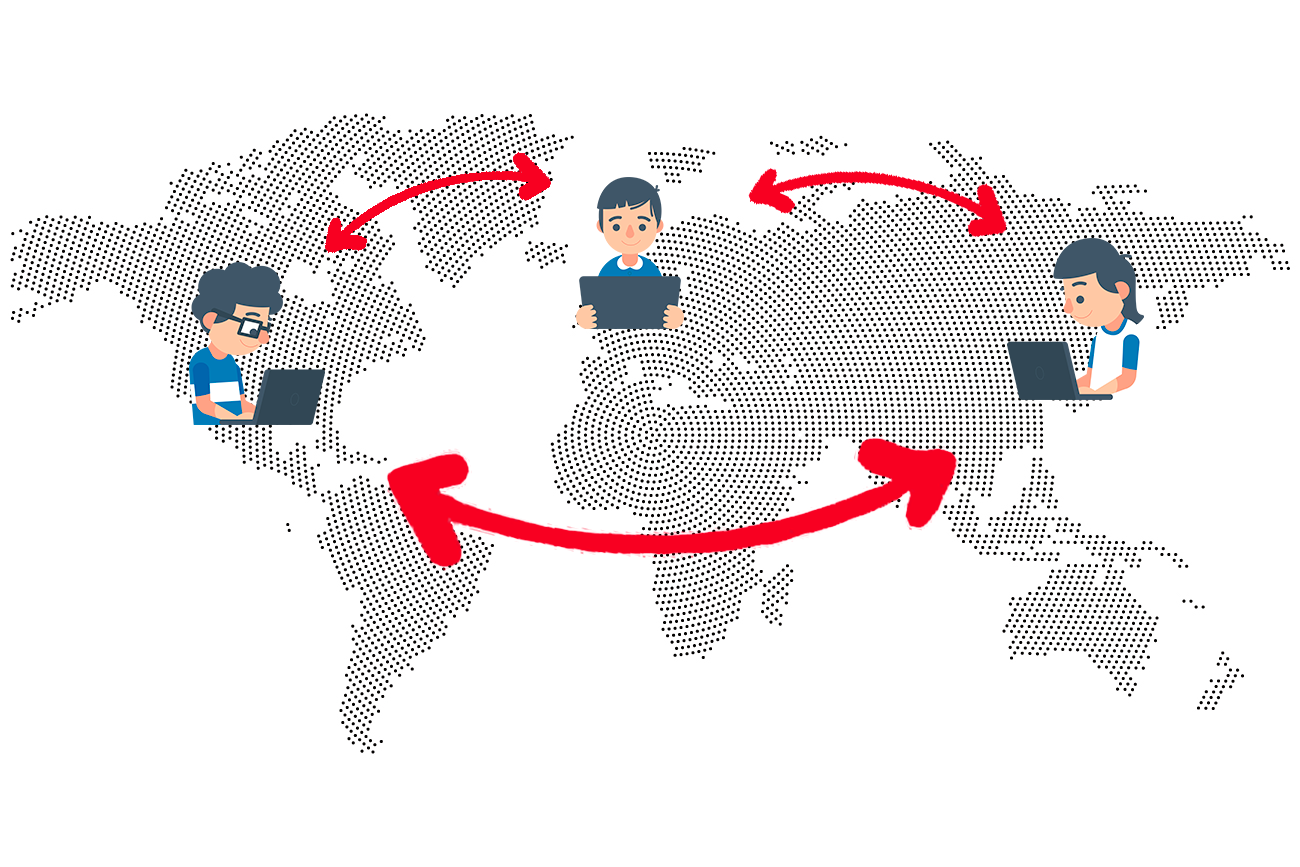
\includegraphics[width=0.75\linewidth]{DGSFiguraMapa}
	\caption[Colaboración mundial en el DGS]{En el DGS diferentes equipos de desarrollo colaboran a nivel mundial en un mismo proyecto}
	\label{fig:DGSFiguraMapa}
\end{figure} 

Gradualmente, esta tendencia esta cogiendo cada vez más fuerza en el campo de la ingeniería del software, considerándose una norma en el desarrollo de software \cite{bosnic2019assessing}. Esto es debido a que las organizaciones pueden conseguir grandes beneficios utilizando este nuevo modelo de desarrollo, ya que la principal ganancia que se consigue con su uso es la reducción en el coste económico de los proyectos, debido a que se suelen buscar territorios donde la mano de obra cualificada es barata y fácilmente disponible \cite{monasor2010preparing}. Además, se pueden encontrar otros beneficios notables como pueden ser el acercamiento del desarrollo del software al cliente y al mercado local, la reducción del período necesario para el desarrollo del software al maximizar la productividad y la expansión hacia la inclusión de trabajadores mayormente cualificados en sus actividades de desarrollo \cite{aagerfalk2008benefits}.

Sin embargo, acompañando a las anteriores ventajas que se pueden conseguir con los proyectos DGS, existen una serie de inconvenientes, los cuales son causados, principalmente, a las diferencias existentes en este tipo de proyectos las cuales podemos dividir en cuatro clases: las \emph{diferencias lingüísticas}, la \emph{distancia geográfica}, la \emph{diferencia cultural} y la coexistencia de diferentes \emph{zonas horarias}; haciendo mucho más difícil el consenso y entendimiento común \cite{monasor2010preparing}. Estas diferencias acentúan la problemática de administrar y gestionar un proyecto software, apareciendo así los tres principales desafíos en la gestión de proyectos DGS (fig.~\ref{fig:desafiosDGS}), también llamado en \cite{piattini2014desarrollo} como las 3 ces:
\begin{itemize}
	\item Desafíos en la comunicación. Los equipos de trabajo deben mantener una comunicación adecuada y activa, con el fin de llevar a cabo un intercambio constante de información y conocimientos. 
	\item Desafíos en la coordinación. Las tareas deben estar sincronizadas, para no sufrir retrasos y alcanzar objetivos e intereses comunes. 
	\item Desafíos en el control. El proyecto debe ser gestionado constantemente y confirmar que se cumplen fechas de entrega, estándares, presupuestos, etc.; además de solventar posibles contratiempos que puedan ocurrir durante el ciclo de vida del proyecto. 
\end{itemize}

\begin{figure}[htb]
	\centering
	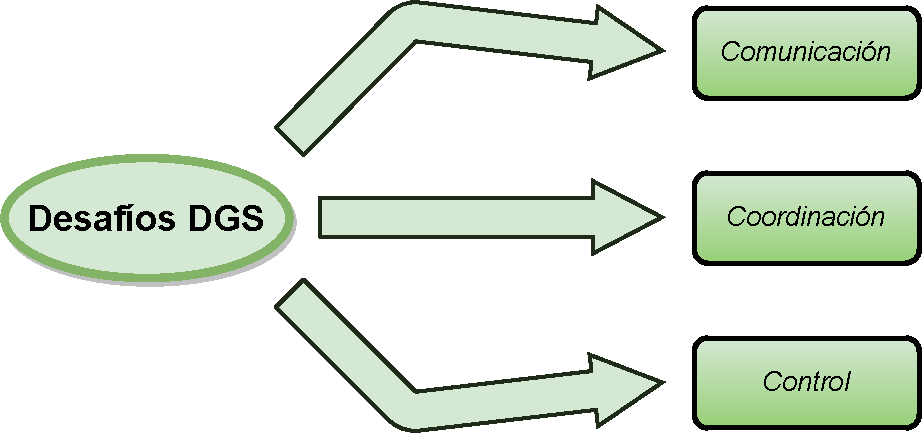
\includegraphics[width=0.75\linewidth]{desafiosDGS}
	\caption[Desafíos en los proyectos DGS]{Los tres principales desafíos en la gestión de proyectos DGS}
	\label{fig:desafiosDGS}
\end{figure}

Estos inconvenientes y desafíos complican la gestión de este tipo de proyectos, lo que puede implicar en retrasos de tareas o incluso en la cancelación del mismo, ya que según la literatura, la mayoría de proyectos DGS terminan fracasando. Según \cite{lino2015project}, la principal causa del elevado fracaso de estos proyectos es debido a la imperfecta y dificultosa gestión de los mismos. Es por esto, que para conseguir los beneficios que nos ofrece el DGS es necesario que los jefes de proyecto posean grandes conocimientos y experiencia en la gestión de estos proyectos, además de contar con una serie de habilidades (no solo técnicas, sino también no técnicas), para hacer frente a los posibles contratiempos que puedan ocurrir en el ciclo de vida del proyecto y conseguir la finalización exitosa del mismo.


\section{Propuesta}
\label{sec:Propuesta}

Como se ha indicado en la sección anterior, existe una gran problemática con la nueva tendencia de desarrollar software mediante un entorno global, debido a que un elevado número de proyectos que utilizan este tipo de modelo de desarrollo terminan fracasando, y son escasos aquellos que consiguen finalizar exitosamente, obteniéndose así los beneficios que se consiguen frente al modelo de desarrollo tradicional. Esta situación se debe, en especial, a que la educación en actividades para enseñar conocimientos sobre DGS no se está teniendo en cuenta, lo que implica que futuros ingenieros de software no posean ciertas habilidades y capacidades necesarias para afrontar los desafíos que conllevan los proyectos DGS \cite{monasor2010preparing}. Es evidente que este modelo de desarrollo se termine convirtiendo en un estándar, por lo que es necesario entrenar a nuestros estudiantes de ingeniería de software para afrontar estas dificultades, ya que se terminarán convirtiendo en los futuros ingenieros de DGS \cite{beecham2017best}.

La gestión y administración es el pilar principal sobre el que gira un proyecto, y en especial un proyecto DGS, ya que es necesaria la organización de un gran número de trabajadores y equipos de desarrollo, a los que se le añade la problemática de gestionar diferentes factores a tener en cuenta como la separación geográfica, la cultura de los diferentes países involucrados en el proyecto o el horario de trabajo en cada país, es por esto que gestionar este tipo de proyectos eficientemente, es un autentico reto. Por lo tanto, es evidente la necesidad de que existan jefes de proyecto altamente cualificados en la gestión de proyectos DGS, para que puedan afrontar la administración del mismo con éxito, solventando todos los impedimentos que puedan ocasionarse. Sin embargo, en la actualidad es complicado encontrar a jefes de proyectos DGS altamente cualificados, con una gran experiencia y con los conocimientos y habilidades necesarias para afrontar correctamente su trabajo. Como consecuencia, son muchas las organizaciones y artículos que han demandado la carencia de habilidades y experiencia en los jefes de proyecto DGS, como la principal causa del elevado nivel de fracaso en los mismos \cite{lino2015project}.

Por consiguiente, es notoria la necesidad de que existan programas de educación que enseñen a nuestro futuros ingenieros de software conocimientos sobre DGS en general, y habilidades (tanto técnicas como no técnicas) necesarias para afrontar con éxito la gestión de este tipo de proyectos en particular. En contraposición, llevar a cabo el entrenamiento y enseñanza de estas habilidades y conocimientos no es una tarea sencilla, puesto que se precisaría la necesidad de introducir a ingenieros de software inexpertos en proyectos reales (para que adquieran esa experiencia necesaria) y por consiguiente las compañías no estén dispuestas a invertir sus recursos en este tipo de programas de entrenamiento. Esta posición de las compañías es debido a que se pueden poner en riesgo proyectos en curso, además de resultar complejo reproducir un escenario real en un entorno de educación \cite{monasor2010preparing}.

En cualquier caso, hay diferentes formas de llevar a cabo la educación de diferentes conocimientos prácticos y el entrenamiento de ciertas habilidades, sin que esto pueda afectar, en nuestro caso, a un proyecto real. En el campo de la \emph{Educación en la Ingeniería de Software} se han realizado avances, buscando la manera más efectiva de educar ciertos conocimientos a estudiantes de ingeniería de software, apareciendo métodos tradicionales como proyectos finales, combinación de diferentes técnicas de enseñanza como aprendizaje basado en proyectos \cite{alabbadi2016proposed}, innovadoras estrategias como las clases volteadas \cite{choi2013applying}, o darle un enfoque relacionado con el uso de juegos, apareciendo el termino de \emph{Gamificación} \cite{connolly2007application}.

Dentro de la gamificación podemos encontrar diferentes tendencias como pueden ser: los cursos académicos \cite{murphy2008distance}, los entornos de aprendizaje \cite{burnell2002teaching} o las aplicaciones que presentan escenarios reales, conocidos como \emph{Juegos Serios} (JSs) \cite{meneely2009preparing}. En especial, los JSs (también llamados juegos educativos), según \cite{calderon2018multivocal}, consisten en juegos que van más allá del puro entretenimiento y constituyen una potente herramienta que permite a sus jugadores experimentar y aprender de sus errores, adquiriendo así experiencia y conocimientos. Los JSs ayudarán en el proceso de aprendizaje mediante la simulación de entornos virtuales, sin el riesgo que conllevaría tener al estudiante en un entorno real \cite{lino2015project, beecham2017best, calderon2018multivocal}, además de que la tendencia del desarrollo de JSs ha tenido una gran aceptación en la última década.

Como resultado de lo cual, este \emph{Trabajo Fin de Carrera} (TFG) se centrará en el desarrollo de un JS, llamado \emph{GLOBAL-MANAGER}. El objetivo de GLOBAL-MANAGER será el de ayudar a estudiante en ingeniería de software a adquirir y entrenar ciertas habilidades (en especial aquellas no técnicas también llamadas \emph{soft skills}) necesarias cuando se aborda el papel de jefe de proyecto DGS. El jugador tendrá que abordar la gestión de un proyecto DGS ficticio desde el comienzo hasta la entrega del producto software al cliente, tratando de resolver los diferentes impedimentos que se puedan ocasionar en el ciclo de vida. De esta manera, los jugadores podrán adquirir experiencia de una manera sencilla, barata e independiente, permitiéndoles afrontar con éxito un futuro trabajo en la gestión de un proyecto DGS.

Este TFG se enmarca dentro de un contrato I+D con el grupo de investigación Alarcos\footnote{\url{https://alarcos.esi.uclm.es}} de la Universidad de Castilla La-Mancha (UCLM)\footnote{\url{https://www.uclm.es/}}, en concreto en el proyecto "G3SOFT: Ingeniería de Modelos para el Gobierno y Gestión del Desarrollo Global de Software"\footnote{\url{https://alarcos.esi.uclm.es/proyectos/G3SOFT/index.php}}, el cual se centra en la mejora del gobierno y la gestión de proyectos de DGS. En la tab.~\ref{tab:ResumenG3SOFT} se muestra un resumen de dicho proyecto.

\begin{table}[htbp]
	\centering
	\setlength{\arrayrulewidth}{0.5mm}
	\arrayrulecolor{white}
	\resizebox{\textwidth}{!}{
    \begin{tabular}{l | p{25.5em}}
        \rowcolor[rgb]{.082, .082, .565} \textcolor[rgb]{1, 1, 1}{\textbf{Nombre:}} & \cellcolor[rgb]{.753, .753, .753}G3SOFT:Ingeniería de Modelos para el Gobierno y Gestión del\newline{}Desarrollo Global de Software \\ \hline
        \rowcolor[rgb]{.082, .082, .565} \textcolor[rgb]{1, 1, 1}{\textbf{Financiación:}} & \cellcolor[rgb]{.753, .753, .753}JJCM Consejería de Educación y Cultura y Deportes, y Fondos\newline{}FEDER \\ \hline
        \rowcolor[rgb]{.082, .082, .565} \textcolor[rgb]{1, 1, 1}{\textbf{Referencia:}} & \multicolumn{1}{l}{\cellcolor[rgb]{.753, .753, .753}SBPLY/17/180501/000150} \\ \hline
        \rowcolor[rgb]{.082, .082, .565} \textcolor[rgb]{1, 1, 1}{\textbf{Dirección WEB:}} & \multicolumn{1}{l}{\cellcolor[rgb]{.753, .753, .753}\url{https://alarcos.esi.uclm.es/proyectos/G3SOFT/index.php}} \\ \hline
        \rowcolor[rgb]{.082, .082, .565} \textcolor[rgb]{1, 1, 1}{\textbf{Grupo de investigación:}} & \multicolumn{1}{l}{\cellcolor[rgb]{.753, .753, .753}Grupo Alarcos} \\ \hline
        \rowcolor[rgb]{.082, .082, .565} \textcolor[rgb]{1, 1, 1}{\textbf{Universidad colaboradora:}} & \multicolumn{1}{l}{\cellcolor[rgb]{.753, .753, .753}Universidad de Castilla-La Mancha (UCLM)} \\ \hline
    	\rowcolor[rgb]{.082, .082, .565} \textcolor[rgb]{1, 1, 1}{\textbf{Investigadores principales:}} & \cellcolor[rgb]{.753, .753, .753}Francisco Ruiz Gónzalez\newline{}Aurora Vizcaíno Barceló \\ \hline
    \end{tabular}}
	\caption{Resumen del proyecto G3SOFT}
	\label{tab:ResumenG3SOFT}
\end{table}

\section{Estructura del documento}
\label{sec:Estructura}
\chapter{Objetivos}
\label{cap:Objetivo}

Este capítulo se centrará en presentar y explicar de manera detallada cual es el objetivo principal que se persigue con la realización del presente TFG, al igual que los objetivos específicos, donde se especificarán aquellos objetivos funcionales y técnicos necesarios para la elaboración del proyecto. A modo de resumen, al final del presente capítulo en la Tabla \ref{tab:ResumenObjetivos}, se mostrarán todos los objetivos que se han definido en el inicio del proyecto.

\section{Objetivo principal}
\label{sec:ObjetivoP}

El principal objetivo (OP) del presente TFG consiste en diseñar y desarrollar una aplicación software de escritorio, la cual consistirá en un JS en \emph{2.5D} (\emph{pseudo-3D}\footnote{\url{https://es.wikipedia.org/wiki/2.5D}}, la tridimensionalidad de un videojuego en 3D se limita a un plano de dos dimensiones), el cual tendrá como objetivo ayudar a estudiantes y profesionales de la ingeniería de software a adquirir ciertas \emph{soft skills}, las cuales son necesarias para llevar a cabo una correcta gestión de un proyecto DGS.

\section{Requisitos específicos funcionales}
\label{sec:ObjetivosF}

El actual proyecto está compuesto por una serie de requisitos específicos funcionales (REFs), los cuales han de tenerse en cuenta en el desarrollo del JS \emph{Global-Manager}. Al final del TFG y en especial en el Capítulo \ref{cap:ConclusionPropuesta}, se llevará a cabo un análisis para comprobar si dichos requisitos han sido debidamente cumplimentados. Estos REFs son los siguientes:

\begin{itemize}
	\item \textbf{REF1.} El JS diferenciará un total de tres niveles distintos de jugador. Estos niveles se calcularán utilizando técnicas de \emph{inteligencia artificial} (IA), en función de los conocimientos del jugador en la gestión de proyectos y en el modelo de desarrollo de software DGS. Los niveles de usuarios que dispondrá el juego serán:
	\begin{itemize}
		\item[-] \textsc{Nivel básico:} Se corresponderá a aquellos jugadores que posean bajos o nulos conocimientos en la gestión de proyectos o en el DGS, además de no tener una gran experiencia en el desarrollo de software. Son aquellas personas que necesitarán un aprendizaje mucho más lento y prolongado para adquirir todos los conocimientos necesarios para la gestión de proyectos DGS.
		\item[-] \textsc{Nivel intermedio:} Se corresponderá a aquellos jugadores que posean ciertos conocimientos en la gestión de proyectos o en el DGS, o incluso poseer cierta experiencia en dichos campos. Estas personas necesitarán de un aprendizaje mucho más rápido, debido a que ya conocerán ciertos aspectos de la materia y les costará menos acostumbrarse al juego.
		\item[-] \textsc{Nivel avanzado:} Se corresponderá a aquellos jugadores que posean grandes conocimientos en la gestión de proyectos o en el DGS, además de haber trabajado en numerosas ocasiones en alguno de estos campos. En este último nivel, los jugadores no necesitarán tanto adquirir conocimientos, sino reforzarlos y entrenarse para mejorar su capacidad de gestionar proyectos DGS satisfactoriamente.
	\end{itemize}
	
	\item \textbf{REF2.} El JS dispondrá de un \emph{modelo de estudiante} dinámico, es decir, se creará a cada jugador un proceso de aprendizaje en función del nivel de jugador que se le haya definido al principio. Por lo tanto, las partidas que juegue dicho jugador se crearán automáticamente personalizadas a sus conocimientos.
	
	\item \textbf{REF3.} Las partidas del juego deberán estar divididas en dos fases. La primera fase consistirá en la configuración inicial del proyecto DGS ficticio, la cual estará compuesta por una interfaz gráfica donde se mostrarán un conjunto de parámetros, los cuales son necesarios conocerlos y configurarlos en un proyecto de estas características. El jugador podrá fijar cada uno de los parámetros. Además, en tiempo real, se calcularán un conjunto de factores de éxito del proyecto con la configuración actual y un nivel de dificultad del proyecto (el cual podrá tener los siguientes valores \emph{muy fácil}, \emph{fácil}, \emph{normal}, \emph{difícil}, \emph{muy difícil}), que ayudará a saber si la configuración definida es correcta.
	
	\item \textbf{REF4.} La segunda fase consistirá en una simulación de un proyecto DGS, en donde el jugador adquirirá el rol de jefe de proyecto y deberá administrar dicho proyecto. El jugador tendrá que hacer frente y en algunas ocasiones solucionar diferentes situaciones, a las cuales llamaremos eventos, que puedan ocurrir en el ciclo de vida de un proyecto DGS real. Estos eventos estarán relacionados con las tres ces (los tres grandes desafíos de un proyecto DGS): comunicación, coordinación y control; y podrán ser tanto eventos positivos (repercusión favorable hacia el proyecto), como eventos negativos (repercusión desfavorable hacia el proyecto).
\end{itemize}


\section{Requisitos específicos no funcionales}
\label{sec:ObjetivosT}

Una vez definidos cuales serán los REFs del proyecto en la Sección \ref{sec:ObjetivosF}, es necesario definir otro tipo de requisitos específicos muchos más técnicos (RENFs). Estos RENFs son los siguientes:

\begin{itemize}
	\item \textbf{RENF1.} En el cálculo del nivel del jugador (anteriormente descrito) se deberán utilizar técnicas de IA, en especial utilizando \emph{Lógica Borrosa}\footnote{La lógica borrosa, también conocida como lógica difusa, consiste en un enfoque computacional basado en grupos de pertenencia(parcialmente verdadero o parcialmente falso), en vez de en la tradicional lógica booleana de verdadero o falso. \url{https://www.wikiversus.com/informatica/logica-difusa/}}. Al principio del juego y antes de que el jugador juegue una partida, deberá rellenar un formulario con diferentes preguntas sobre sus conocimientos y experiencia en gestión de proyectos y DGS. A través de estas preguntas se obtendrá un nivel para el nuevo jugador. Para implementar esta encuesta y el cálculo automático del nivel se llevará a cabo una entrevista a un experto en la materia, para adquirir aquellos conocimientos que nos hagan saber cuales son los aspectos importantes para conocer las nociones sobre gestión de proyectos y DGS de una persona.
	
	\item \textbf{RENF2.} Desarrollar el JS utilizando el marco de trabajo de Microsoft \emph{.NET}\footnote{\url{https://dotnet.microsoft.com/}}. Además, se utilizará el lenguaje de programación \emph{C\#}\footnote{https://es.wikipedia.org/wiki/C\_Sharp}, el cual se encuentra más enfocado en la programación de videojuegos.
	
	\item \textbf{RENF3.} La gestión de los datos asociados al proyecto (características de los eventos, modelo del estudiante y dominio) se llevará a cabo utilizando el sistema de gestión de bases de datos relacional \emph{SQLite}\footnote{https://sqlite.org/index.html}, junto con el componente \emph{LINQ}\footnote{https://docs.microsoft.com/es-es/dotnet/csharp/programming-guide/concepts/linq/introduction-to-linq-queries} (Language Integrated Query) de Microsoft .NET para las consultas a datos de manera nativa a los lenguajes .NET, como C\#.
\end{itemize}

\clearpage

\begin{table}[!th]
		\setlength{\arrayrulewidth}{0.3mm}
		\arrayrulecolor{black}
		\resizebox{\textwidth}{!}{
		\begin{tabular}{|l|p{15cm}|}
			\hline
			\rowcolor[HTML]{EFEFEF} 
			\multicolumn{1}{|c|}{\cellcolor[HTML]{EFEFEF}{\color[HTML]{000000} \textit{\textbf{Código Objetivo}}}} & \multicolumn{1}{c|}{\cellcolor[HTML]{EFEFEF}{\color[HTML]{000000} \textit{\textbf{Descripción}}}}                                                                                                                                                                                                                                           \\ \hline
			\rowcolor[HTML]{9AFF99} 
			{\color[HTML]{000000} \textbf{OP}}                                                                     & {\color[HTML]{000000} Diseño y desarrollo de un JS en 2.5D, que ayude a sus jugadores a adquirir ciertas soft skills y a entrenarse en la correcta gestión de proyectos DGS.}                                                                                                                                                               \\ \hline
			\rowcolor[HTML]{FFCE93} 
			{\color[HTML]{000000} \textbf{REF1}}                                                                   & {\color[HTML]{000000} Diferenciación de tres niveles de jugador (bajo, medio y alto) para crear asi diferentes procesos de aprendizaje, en función de los conocimientos del jugador en la mataria.}                                                                                                                                         \\ \hline
			\rowcolor[HTML]{FFCE93} 
			{\color[HTML]{000000} \textbf{REF2}}                                                                   & {\color[HTML]{000000} Creación de un modelo de estudiante dinámico para la creación de partidas personalizadas.}                                                                                                                                                                                                                            \\ \hline
			\rowcolor[HTML]{FFCE93} 
			{\color[HTML]{000000} \textbf{REF3}}                                                                   & {\color[HTML]{000000} Primera fase del juego: Implementación de una interfaz grafica, en donde el jugador deberá configurar un conjunto de parametros iniciales del proyecto DGS. Además del calculo, en tiempo real, de un conjunto de fáctores de éxito y el nivel de dificultad del proyecto.}                                           \\ \hline
			\rowcolor[HTML]{FFCE93} 
			{\color[HTML]{000000} \textbf{REF4}}                                                                   & {\color[HTML]{000000} Segunda fase del juego: Implementación de la simulación del proyecto en función de la configuración inicial definida, el jugador deberá gestionar dicho proyecto DGS haciendo frente a diferentes eventos (positivos y negativos) relacionados con la comunicación, coordinación y control del proyecto.}             \\ \hline
			\rowcolor[HTML]{CBCEFB} 
			{\color[HTML]{000000} \textbf{RENF1}}                                                                   & {\color[HTML]{000000} Cálculo del nivel del jugador mediante un formulario, el cual se implementará utilizandológica borrosa, tras realizar una adquisición de conocimientos mediante una entrevista a un experto sobre cuales son los aspectos más importantes para conocer las nociones sobre gestión de proyectos y DGS de una persona.} \\ \hline
			\rowcolor[HTML]{CBCEFB} 
			{\color[HTML]{000000} \textbf{RENF2}}                                                                   & {\color[HTML]{000000} Desarrollo del JS utilizando Microsoft .NET, junto con el lenguaje de programación C\#.}                                                                                                                                                                                                                              \\ \hline
			\rowcolor[HTML]{CBCEFB} 
			{\color[HTML]{000000} \textbf{RENF3}}                                                                   & {\color[HTML]{000000} Gestión de los datos asociados al proyecto mediante el sistema de gestión de bases de datos relacionales SQLite, junto con el componente LINQ de Microsoft .NET.}                                                                                                                                                     \\ \hline
		\end{tabular}}
		\caption{Objetivos principal y específicos del presente TFG}
		\label{tab:ResumenObjetivos}
	\end{table}
\chapter{Estado del arte}
\label{cap:Antecedentes}

El objetivo de este capítulo consistirá en la definición y explicación detallada del argumento del presente TFG. A continuación, se presenta el estado del arte del método de desarrollo DGS, donde se detallará su definición, beneficios, problemáticas. Además, se indicará la importancia que conlleva la gestión en un proyecto de estas características. Por otra parte, se harán referencia a las habilidades que son necesarias para llevar a cabo el trabajo de jefe de proyecto en un entorno DGS. A continuación, se tratará la situación actual de la gamificación para la enseñanza, junto con los JS y el uso de la IA para la personalización de juegos. Para finalizar, se listarán una serie de ejemplos relacionados con el objetivo de este TFG.

\section{Desarrollo Global del Software}
\label{sec:DGS}

Debido a la globalización, en el campo de la ingeniería de software aparece un nuevo modelo de desarrollo denominado como Desarrollo Global de Software. A diferencia del modelo tradicional, donde el equipo de trabajo estaba centralizado en un solo edificio o en varios edificios, pero siempre en el mismo país, el DGS consiste en el desarrollo de un producto o servicio software, en donde diferentes equipos de desarrollo, pertenecientes a organizaciones diferentes y ubicadas en países dispares, colaboran en el mismo proyecto software y son coordinados y gestionados en tiempo real basándose en los desafíos del DGS, las 3Cs: comunicación, coordinación y control \cite{piattini2014desarrollo}.

A lo largo de la última década, el DGS se ha afianzado como una de las vertientes más relevantes en la investigación y práctica dentro del campo de la ingeniería del software. Las primeras prácticas de este nuevo tipo de proceso de desarrollo de software surgen hace más de 30 años, con los primeros usos de \emph{outsourcing} \cite{boehm2006view}. Sin embargo, no sería hasta 2006 cuando se extendiera su uso con la celebración de la primera conferencia internacional sobre DGS, el \emph{ICGSE} (\emph{IEEE International Conference on Global Software Engineering}) \cite{piattini2014desarrollo, vizcaino2015vision}.

\subsection{Beneficios del Desarrollo Global del Software}
\label{sec:Beneficios}

Cuando hablamos de DGS es notable resaltar la cantidad de beneficios que pueden alcanzar las empresas con su correcto uso. Sin embargo, no todos sus beneficios son conocidos en el sector, ya que podemos encontrar beneficios que se puedan obtener de forma directa o indirecta, y son muchas las investigaciones, como \cite{aagerfalk2008benefits, conchuir2009global, conchuir2006exploring, vizcaino2015vision}, que están estudiado tanto aquellos beneficios notables como aquellos no vistos a simple vista con el uso de DGS como proceso de desarrollo de software. Por lo tanto, a continuación se formulará un listado de todos los beneficios que podemos obtener con esta nueva tendencia:

\begin{itemize}
	\item \textbf{Reducción del coste de producción.} Uno de los beneficios más importantes y una de las razones por las cuales las organizaciones y compañías están optando en afrontar un modelo de desarrollo de software global, consiste en la reducción de los costes del proyecto en el proceso de producción. Este beneficio se debe en gran medida a la globalización, ya que ha hecho posible que actividades en el proceso de desarrollo puedan realizarlas empleados que se encuentran en países que cuentan con salarios más reducidos \cite{aagerfalk2008benefits}. Un ejemplo de esta situación sería la India, en donde el salario base anual de un desarrollador de software es de \emph{US\$15,000}, mientras que en Irlanda un mismo trabajador puede ganar cuatro veces esa cantidad, y a su vez esa cantidad consistiría en la mitad del salario de un desarrollador en Estados Unidos \cite{conchuir2009global, conchuir2006exploring}. Alcanzar esta situación también ha sido posible gracias al despliegue de enlaces de comunicación de alta velocidad, los cuales ayudan a la transferencia de información y conocimientos entre los empleados separados geográficamente \cite{aagerfalk2008benefits}. Este beneficio conlleva que las compañías tengan que tener en cuenta la gestión del coste en cuanto a los viajes de empleados entre grupos de trabajo, ya que en este modelo de desarrollo los empleados no se conocen y es necesario que exista un poco de comunicación \emph{face-to-face} para consolidar la relación entre empleados, creando así un ambiente de confianza \cite{conchuir2009global, conchuir2006exploring}.
	
	\item \textbf{Aprovechamiento de la zona horaria.} En un entorno global, como es un proyecto que utiliza DGS como proceso de desarrollo, hace posible que las organizaciones puedan aprovecharse de la diferencia en las zonas horarias de sus empleados, con el fin de incrementar las horas de trabajo del día y reducir así el tiempo de desarrollo del servicio o producto software \cite{conchuir2006exploring, conchuir2009global}. De esta manera se lograrán jornadas de trabajo más extensas en el proyecto, que en uno con un modelo tradicional y por lo tanto una mayor productividad para finalizar dicho proyecto en un menor tiempo \cite{vizcaino2015vision}. Esta situación es conocida como desarrollo \emph{follow-the-sun}\footnote{"La estrategia follow-the-sun se caracteriza en que cuando un equipo de trabajo finaliza su jornada laboral, la jornada de otro equipo comienza en otra parte del mundo, de esta manera se consigue un desarrollo del proyecto las 24 horas del día" \cite{piattini2014desarrollo}} y es considerada un potente beneficio en el DGS. Sin embargo, lograr este escenario en la realidad es complicado, además de poder producirse retrasos en las respuestas en la comunicación de los empleados, debido a horarios de comida o días festivos, lo que puede ocasionar retrasos en el proyecto. Por lo tanto, es importante que exista cierto solapamiento en las jornadas laborales de los empleados, con el fin de que exista cierta comunicación sincrona \cite{conchuir2006exploring, conchuir2009global}.
	
	\item \textbf{Modularización del proceso de desarrollo.} Una manera de afrontar un proyecto DGS es separando las tareas del proyecto en módulos independientes bien definidos, para que de esta manera cada equipo de desarrollo posea ciertos módulos de trabajo. Permitiendo así que las decisiones referentes a cada módulo se tomen de forma aislada entre los miembros del equipo de trabajo, además de reducir costes en la coordinación. De esta manera, podemos diferenciar dos tipos de estrategias: \emph{basada en módulos}\footnote{"La estrategia basada en módulos consiste en dividir el proyecto en diferentes módulos, los cuales se pueden considerar un artefacto completo del proyecto, y repartirlos entre los sites" \cite{piattini2014desarrollo}} y \emph{basada en fases}\footnote{"La estrategia basada en fases consiste en asignar a cada equipo de trabajo una fase del proceso de desarrollo software" \cite{piattini2014desarrollo}} \cite{conchuir2006exploring, conchuir2009global, aagerfalk2008benefits}.
	
	\item \textbf{Acceso a plantillas de trabajadores altamente cualificados.} El DGS hace posible acceder fácilmente a grupos de trabajadores altamente cualificados repartidos por todo el mundo. De esta manera, las empresas se pueden beneficiar de los conocimientos, diversidad de experiencias, destrezas y habilidades de trabajadores repartidos por todo el mundo, para que lleven a cabo el desarrollo de diferentes actividades software del proyecto DGS \cite{vizcaino2015vision, conchuir2006exploring, conchuir2009global, aagerfalk2008benefits}.
	
	\item \textbf{Proximidad al cliente y a su mercado.} Gracias al DGS, las compañías pueden establecer fácilmente filiales en aquellos países donde se localizan los clientes, y conseguir así un acercamiento y un conocimiento más profundo del mercado local. Además, con esta practica las compañías consiguen expandirse hacia nuevos mercados, sin la necesidad de trasladar a sus equipos de desarrolladores \cite{vizcaino2015vision, conchuir2006exploring, conchuir2009global, aagerfalk2008benefits}.
\end{itemize}

\subsection{Desafíos del Desarrollo Global del Software}
\label{sec:Desafios}

La distancia existente entre los equipos de desarrolladores en un proyecto DGS hace posible el acercamiento hacia grandes beneficios por parte de las organizaciones, sin embargo conseguirlos no es tarea sencilla, ya que dicha distancia conlleva también la introducción de un conjunto de desafíos, a los cuales, las organizaciones deben hacer frente para alcanzar los beneficios anteriormente citados \cite{conchuir2006exploring}. Los desafíos que puedan aparecer en este tipo de proyectos se pueden agrupar en relación con los tres grandes procesos en el desarrollo de software: comunicación, coordinación y control. Estos grupos de desafíos también se les conoce como las 3 Cs \cite{vizcaino2015vision, piattini2014desarrollo}, y hacen referencia a las siguientes situaciones:

\begin{itemize}
	\item \textbf{Desafíos de comunicación.} Hace referencia a aquellas situaciones en donde se lleva a cabo una comunicación entre trabajadores, es decir, un intercambio de información y conocimientos con el fin de que no se produzcan malentendidos y el proyecto pueda avanzar.
	\item \textbf{Desafíos de coordinación.} Hace referencia al mantenimiento de los trabajadores en la realización de las diferentes tareas de un proyecto, con el fin de alcanzar objetivos e intereses comunes y la evolución del proyecto progrese adecuadamente.
	\item \textbf{Desafíos de control.} Hace referencia a la administración y gestión del proyecto en general, teniendo en cuenta día a día diferentes aspectos del proyecto como pueden ser los calendarios de entregas, presupuestos, calidad, estándares, etc. 
\end{itemize}

Por otro lado, los proyectos DGS se caracterizan por la existencia de diferentes nacionalidades, organizaciones e inclusos culturas que pueden agravar esta situación. Esto hace que puedan aparecer diferentes tipos de distancias entre los miembros del proyecto, provocando una acentuación en los desafíos anteriormente citados \cite{vizcaino2015vision}. De esta manera, aparece otra clasificación de los desafíos de un proyecto DGS en función de lo que se conoce en la literatura como las tres distancias \cite{vizcaino2015vision, conchuir2006exploring, conchuir2009global}:

\begin{itemize}
	\item \textbf{Distancia geográfica.} Se puede definir como la medida de esfuerzo necesario en un individuo para visitar un punto alejado de su ubicación. Un ejemplo sería el de dos ubicaciones separadas geográficamente por una gran distancia pero con un enlace aéreo directo frente a dos ubicaciones cercanas geográficamente pero con poca infraestructura de transporte; de esta manera el primer caso poseerá poca distancia geográfica, mientras que en el segundo será elevada \cite{vizcaino2015vision}. Además, la distancia geográfica dificulta la posibilidad de existir una comunicación informal o cara a cara entre los miembros que ayude a afianzar las relaciones entre ellos, el trabajo en equipo, consolidación de la confianza y la comunicación fluida de información importante del proyecto \cite{conchuir2006exploring}.
	
	\item \textbf{Distancia temporal.} Ligada a la anterior, se puede definir como la medida de la diferencia en el tiempo existente en la comunicación entre dos individuos \cite{vizcaino2015vision}. Como se dijo en la sección anterior, la distancia temporal en un proyecto DGS puede conllevar ciertos desafíos como es la estrategia follow-the-sun, con el objetivo de reducir tiempo y costes, sin embargo, surgen también ciertas problemáticas como es el hecho de que aparezcan retrasos en las respuestas en los intercambios de información entre los trabajadores, debido a la reducción del solapamiento de horas en las jornadas laborales de los equipos de desarrolladores. Esto implica que se tengan que usar herramientas de comunicación asíncronas, las cuales pueden afectar negativamente al manejo de ambigüedades y al aumento de los malentendidos, produciéndose así retrasos en el proyecto; frente a una comunicación síncrona mucho más directa y segura \cite{conchuir2006exploring}.
	
	\item \textbf{Distancia socio-cultural.} Se puede definir como la medida en que un individuo conoce y comprende las costumbres, cultura e idioma de otro individuo, con el objetivo de llevar a cabo una correcta comunicación. Esta situación es debida a que como en un proyecto coexisten diferentes nacionalidades, es frecuente que existan diferentes culturas entre sus miembros \cite{vizcaino2015vision}. Dicha distancia puede conllevar diferentes interpretaciones en una comunicación o situación, lo que puede obstaculizar la comunicación y coordinación del proyecto \cite{conchuir2006exploring}. Además, puede provocar que aparezcan conflictos y malentendidos entre los miembros del proyecto, retrasando así la evolución del mismo.
\end{itemize}

Por lo tanto, es importante tener en cuenta los posibles desafíos que puedan surgir en un proyecto DGS, es por ello que son numerosas las investigaciones sobre estas problemáticas, como es el caso de \cite{niazi2016challenges}, en donde se lleva a cabo una Revisión Sistemática de la Literatura (RSL) de 101 estudios sobre las dificultades más importantes en un proyecto de estas características, junto con un cuestionario a 41 organizaciones sobre sus prácticas en el mundo real. A continuación, utilizando como referencia el estudio de \cite{niazi2016challenges}, se mostrará en la Tabla \ref{tab:DificultadesDGS} las frecuencias de importancia para las dificultades, que se deben afrontar en los proyectos DGS, en 101 estudios (tab. 3, pág. 5) y para 41 organizaciones (tab. 6, pág. 7), junto con una media ponderada de ambos valores.

\begin{table}[htbp]
  \centering
  \resizebox{\textwidth}{!}{
    \begin{tabular}{lccc|}
    \rowcolor[rgb]{ .851,  .851,  .851} \multicolumn{1}{c}{\textbf{Desafío DGS}} & \multicolumn{1}{p{12em}}{\textbf{Frequencia de aparición \newline{}en 101 estudios (\%)}} & \multicolumn{1}{p{12.93em}}{\textbf{Frecuencia de acuerdo \newline{}con 41 organizaciones (\%)}} & \textbf{Media (\%)} \\
        \rowcolor[rgb]{ .949,  .949,  .949} \textit{Falta de entendimiento cultural} & \cellcolor[rgb]{ 1,  1,  1}62 & \cellcolor[rgb]{ 1,  1,  1}70 & \cellcolor[rgb]{ 1,  1,  1}\textbf{66} \\
        \rowcolor[rgb]{ .949,  .949,  .949} \textit{Ausencia de comunicación} & \cellcolor[rgb]{ 1,  1,  1}54 & \cellcolor[rgb]{ 1,  1,  1}76 & \cellcolor[rgb]{ 1,  1,  1}\textbf{65} \\
        \rowcolor[rgb]{ .949,  .949,  .949} \textit{Falta de la gestión del conocimiento} & \cellcolor[rgb]{ 1,  1,  1}38 & \cellcolor[rgb]{ 1,  1,  1}78 & \cellcolor[rgb]{ 1,  1,  1}\textbf{58} \\
        \rowcolor[rgb]{ .949,  .949,  .949} \textit{Falta de gestión del tiempo} & \cellcolor[rgb]{ 1,  1,  1}42 & \cellcolor[rgb]{ 1,  1,  1}71 & \cellcolor[rgb]{ 1,  1,  1}\textbf{56.5} \\
        \rowcolor[rgb]{ .949,  .949,  .949} \textit{Ausencia de coordinación} & \cellcolor[rgb]{ 1,  1,  1}35 & \cellcolor[rgb]{ 1,  1,  1}69 & \cellcolor[rgb]{ 1,  1,  1}\textbf{52} \\
        \rowcolor[rgb]{ .949,  .949,  .949} \textit{Ausencia de control} & \cellcolor[rgb]{ 1,  1,  1}27 & \cellcolor[rgb]{ 1,  1,  1}75 & \cellcolor[rgb]{ 1,  1,  1}\textbf{51} \\
        \rowcolor[rgb]{ .949,  .949,  .949} \textit{Actividades de ingeniería de requisitos} & \cellcolor[rgb]{ 1,  1,  1}28 & \cellcolor[rgb]{ 1,  1,  1}71 & \cellcolor[rgb]{ 1,  1,  1}\textbf{49.5} \\
        \rowcolor[rgb]{ .949,  .949,  .949} \textit{Asignación de tareas} & \cellcolor[rgb]{ 1,  1,  1}18 & \cellcolor[rgb]{ 1,  1,  1}80 & \cellcolor[rgb]{ 1,  1,  1}\textbf{49} \\
        \rowcolor[rgb]{ .949,  .949,  .949} \textit{Ausencia de la verdad} & \cellcolor[rgb]{ 1,  1,  1}34 & \cellcolor[rgb]{ 1,  1,  1}59 & \cellcolor[rgb]{ 1,  1,  1}\textbf{46.5} \\
        \rowcolor[rgb]{ .949,  .949,  .949} \textit{Actividades de gestión del cambio} & \cellcolor[rgb]{ 1,  1,  1}22 & \cellcolor[rgb]{ 1,  1,  1}68 & \cellcolor[rgb]{ 1,  1,  1}\textbf{45} \\
        \rowcolor[rgb]{ .949,  .949,  .949} \textit{Falta en la concienciación de equipo} & \cellcolor[rgb]{ 1,  1,  1}23 & \cellcolor[rgb]{ 1,  1,  1}66 & \cellcolor[rgb]{ 1,  1,  1}\textbf{44.5} \\
        \rowcolor[rgb]{ .949,  .949,  .949} \textit{Gestión de conflictos} & \cellcolor[rgb]{ 1,  1,  1}17 & \cellcolor[rgb]{ 1,  1,  1}71 & \cellcolor[rgb]{ 1,  1,  1}\textbf{44} \\
        \rowcolor[rgb]{ .949,  .949,  .949} \textit{Estimación del coste y del esfuerzo} & \cellcolor[rgb]{ 1,  1,  1}15 & \cellcolor[rgb]{ 1,  1,  1}73 & \cellcolor[rgb]{ 1,  1,  1}\textbf{44} \\
        \rowcolor[rgb]{ .949,  .949,  .949} \textit{Actividades de integración} & \cellcolor[rgb]{ 1,  1,  1}14 & \cellcolor[rgb]{ 1,  1,  1}73 & \cellcolor[rgb]{ 1,  1,  1}\textbf{43.5} \\
        \rowcolor[rgb]{ .949,  .949,  .949} \textit{Gestión del riesgo} & \cellcolor[rgb]{ 1,  1,  1}15 & \cellcolor[rgb]{ 1,  1,  1}71 & \cellcolor[rgb]{ 1,  1,  1}\textbf{43} \\
        \rowcolor[rgb]{ .949,  .949,  .949} \textit{Distancia geográfica} & \cellcolor[rgb]{ 1,  1,  1}28 & \cellcolor[rgb]{ 1,  1,  1}56 & \cellcolor[rgb]{ 1,  1,  1}\textbf{42} \\
        \rowcolor[rgb]{ .949,  .949,  .949} \textit{Ausencia de un proceso uniforme entre los diferentes sites} & \cellcolor[rgb]{ 1,  1,  1}19 & \cellcolor[rgb]{ 1,  1,  1}63 & \cellcolor[rgb]{ 1,  1,  1}\textbf{41} \\
        \rowcolor[rgb]{ .949,  .949,  .949} \textit{Falta de una infraestructura informatica adecuada} & \cellcolor[rgb]{ 1,  1,  1}11 & \cellcolor[rgb]{ 1,  1,  1}68 & \cellcolor[rgb]{ 1,  1,  1}\textbf{39.5} \\
        \rowcolor[rgb]{ .949,  .949,  .949} \textit{Protección de la propiedad intelectual} & \cellcolor[rgb]{ 1,  1,  1}9 & \cellcolor[rgb]{ 1,  1,  1}64 & \cellcolor[rgb]{ 1,  1,  1}\textbf{36.5} \\
    \end{tabular}}
  \caption{Frecuencia de la importancia de diferentes dificultades en proyectos DGS}
  \label{tab:DificultadesDGS}
\end{table}

\subsection{Rol del jefe de proyecto}
\label{sec:ImportanciaJP}

La tarea de administración y gestión de un proyecto consiste en el uso de un conjunto de técnicas y herramientas con el objetivo de controlar los recursos de un proyecto y la correcta realización de las diferentes tareas de los miembros, para conseguir así una evolución constante y sin problemas en el desarrollo del servicio o producto software. Dicha tarea esta ligada a diferentes aspectos relevantes de un proyecto, como es la gestión del tiempo, el coste, la calidad y muchos otros. Por lo tanto, el rol de jefe de proyecto es de suma importancia, ya que controlará la consistencia y evolución del proyecto, además de asegurarse de que los objetivos y propósito del mismo se cumplan correctamente y sin incidencias. El jefe de proyecto deberá hacer frente a cualquier contratiempo que pueda surgir a lo largo del proceso de desarrollo del software \cite{colomo2014project}. Cabe destacar, que en la literatura se considera al proceso de gestionar un proyecto software una tarea esencial para alcanzar el éxito, sin embargo, también se considera dicho proceso como una tarea no sencilla, en la cual se necesitan grande conocimientos, habilidades y experiencia en el desarrollo de proyectos, según \cite{boehm1989theory} lo definió como la integración de la tecnología del software, la economía y las relaciones laborales en el contexto de un proyecto software. 

Por otro lado, si hablamos de la gestión de proyectos en un entorno global como es un proyecto DGS, dicha labor se complica aún más. Con la separación de los equipos de desarrolladores de un mismo proyecto en diferentes ubicaciones con sus diferencias temporales, culturales y lingüísticas, implica que el rol de jefe de proyectos DGS sea mucho más complicado, siendo necesaria la organización de trabajadores no conocidos personalmente a diferentes tareas, junto con la gestión de recursos ubicados en distintos lugares del mundo. Adicionalmente, dicha tarea se agrava con los desafíos en las llamadas 3 Ces, comunicación, coordinación y control, siendo un gran número los aspectos y desafíos que debe afrontar un jefe de proyectos DGS con el objetivo de alcanzar exitosamente la correcta colaboración entre los equipos de desarrolladores y la entrega del servicio o producto software al cliente. Debido a esta problemática, es necesaria una profunda educación a los estudiantes de ingeniería de software y a los futuros jefes de proyectos DGS tanto en este nuevo modelo de desarrollo de software como en el proceso más importante en este tipo de proyectos. Por lo que, será necesario un entrenamiento y enseñanza de aquellas habilidades, no solo técnicas, sino en especial aquellas no-técnicas (\emph{soft skills}) necesarias para afrontar con éxito los posibles desafíos que puedan surgir en un proyecto DGS.

\section{Habilidades necesarias en Desarrollo Global del Software}
\label{sec:HabilidadesDGS}

Como hemos dicho anteriormente, trabajar en un entorno distribuido como es un proyecto DGS, resulta complicado, ya que aparecen nuevas situaciones problemáticas debido a las dificultades en la comunicación y en la separación geográfica, temporal y socio-cultural. Además, en el proceso de gestión del proyecto esta situación se agrava siendo necesarios más conocimientos para cumplir correctamente con su trabajo. Por lo tanto, son necesarias ciertas habilidades para trabajar en dichas situaciones. Aunque, ambas, habilidades técnicas y no-técnicas son igual de importantes en un proyecto software, cabe destacar que las habilidades no-técnicas resultan ser más difíciles a la hora de enseñarlas y/o aprenderlas. Por lo tanto, en esta sección nos centraremos en listar y explicar cuales son las habilidades no-técnicas más importantes y necesarias cuando se trabaja en un entorno de desarrollo distribuido y cuando se lleva a cabo la labor de jefe de proyecto.

\subsection{Habilidades en el equipo de trabajo de Desarrollo Global del Software}
\label{sec:HabilidadesT}

Al igual que se citó anteriormente, el elevado nivel de fracaso en los proyectos DGS es debido a la falta de habilidades y competencias relacionadas con este nuevo modelo de desarrollo entre sus trabajadores. Es por esto, que son numerables los estudios que intentan recopilar el conjunto de habilidades necesarias para trabajar en un entorno DGS. Algunos de estos estudios son los siguientes:

En primer lugar, según \cite{bosnic2019assessing}, algunas de las habilidades más útiles en el desarrollo de software son \emph{hablar un idioma extranjero (en especial el inglés)}, \emph{capacidad de tener una cooperación local} y \emph{ser capaz de tomar decisiones}. En adicción a las anteriores, en un entorno distribuido se hacen necesarias nuevas habilidades como \emph{ser capaz de mantener una cooperación remota}, \emph{llevar a cabo una cooperación intercultural} y \emph{una cooperación con el cliente}.

Por otra parte, y de acuerdo con \cite{monasor2010training}, algunas de las habilidades que se deben promover en el entrenamiento de DGS son \emph{ser conscientes de todos los problemas posibles}, \emph{dominar protocolos para la correcta comunicación entre trabajadores (en especial con el uso de ordenadores)}, \emph{correcta comunicación oral y escrita a través de un idioma común}, \emph{conocer los códigos de ética de la organización} y \emph{llevar a cabo una correcta gestión del tiempo}.

En \cite{paasivaara2013teaching}, los autores indican que las habilidades más importantes que deben enseñarse para aprender a trabajar en DGS son \emph{comunicación regular entre los miembros de los equipos de desarrolladores distribuidos}, \emph{contribuir a la dinámica del equipo de trabajo}, \emph{saber como trabajar en equipos culturalmente divergentes}, \emph{gestión del tiempo} y \emph{saber trabajar con tecnologías de colaboración}.

Igualmente, un marco de trabajo para enseñar algunas habilidades de DGS se describe en \cite{damian2006instructional}; las principales habilidades consideradas son \emph{saber comunicarse mediante ordenadores}, \emph{desarrollo iterativo en las relaciones cliente-desarrollador a distancia} y \emph{gestión distribuida de proyectos}.

Por último, el modelo de competencias especificado en \cite{saldana2014skills} indica que las habilidades necesarias en un entorno DGS se pueden dividir en cuatro grupos, dependiendo del rol que se posee en el proyecto, estos roles pueden ser \emph{ingeniero de software}, líder de equipo, \emph{gestor de proyecto} y gerente de la unidad organizadora. Las habilidades que se señalan como necesarias en el entrenamiento de ingenieros de software DGS son \emph{comunicación síncrona y asíncrona}, \emph{identificación  y gestión de las necesidades del proyecto}, \emph{capacidad de solventar problemas técnicos}, \emph{conocimiento de técnicas avanzadas de comunicación distribuida}, \emph{capacidad de autoaprendizaje}, \emph{capacidad de mantener relaciones internacionales}, \emph{uso de tecnologías de la comunicación y la información}, \emph{capacidad de trabajar en un entorno global} y \emph{saber mantener una comunicación oral y escrita en inglés}.

Teniendo en cuenta todas las habilidades y competencias citadas anteriormente encontradas en la literatura, se muestra en la Tabla \ref{tab:SoftSkillsDGS} un resumen de aquellas soft skills más importantes para aprender a la hora de trabajar en un entorno DGS.

\begin{table}[htbp]
  \centering
  \resizebox{\textwidth}{!}{
    \begin{tabular}{lp{33.5em}c}
    	\rowcolor[rgb]{ .851,  .851,  .851} \multicolumn{1}{c}{\textbf{Soft Skills}} & \multicolumn{1}{c}{\textbf{Descripción de la soft skill}} & \textbf{Referencias} \\
        \rowcolor[rgb]{ .949,  .949,  .949} \multicolumn{1}{p{14.43em}}{\textit{Comunicación oral y escrita \newline{}en Inglés}} & \cellcolor[rgb]{ 1,  1,  1}Saber comunicarse oralmente y por escrito con los diferentes miembros de los equipos de trabajo en un idioma común, en especial el Inglés & \cellcolor[rgb]{ 1,  1,  1}\cite{bosnic2019assessing, monasor2010training, saldana2014skills} \\
        \rowcolor[rgb]{ .949,  .949,  .949} \multicolumn{1}{p{14.43em}}{\textit{Comunicación regular entre\newline{}los miembros de los equipos\newline{}de desarrolladores distribuidos}} & \cellcolor[rgb]{ 1,  1,  1}Mantener una comunicación fluida con los diferentes miembros de los equipos distribuidos, sabiendo en cada caso cuál es el mejor protocolo a utilizar (síncrono o asíncrono) y utilizando técnicas avanzadas & \cellcolor[rgb]{ 1,  1,  1}\cite{monasor2010training, paasivaara2013teaching, damian2006instructional, saldana2014skills} \\
        \rowcolor[rgb]{ .949,  .949,  .949} \multicolumn{1}{p{14.43em}}{\textit{Toma de decisiones y resolución\newline{}de problemas}} & \cellcolor[rgb]{ 1,  1,  1}Ser capaz de tomar las decisiones adecuadas para resolver los problemas técnicos que afectan directa o indirectamente a la evolución del proyecto, considerando todas las problemáticas posibles & \cellcolor[rgb]{ 1,  1,  1}\cite{bosnic2019assessing, monasor2010training, saldana2014skills} \\
        \rowcolor[rgb]{ .949,  .949,  .949} \textit{Gestión del tiempo} & \cellcolor[rgb]{ 1,  1,  1}Gestionar el tiempo empleado en el desarrollo de las tareas de los diferentes equipos de trabajo, en un esfuerzo por evitar problemas en el proyecto & \cellcolor[rgb]{ 1,  1,  1}\cite{monasor2010training, paasivaara2013teaching, damian2006instructional} \\
        \rowcolor[rgb]{ .949,  .949,  .949} \textit{Cooperación remota} & \cellcolor[rgb]{ 1,  1,  1}Colaborar tanto entre los miembros del mismo equipo como entre los diferentes equipos de trabajo para dinamizar el proyecto, utilizando también herramientas y tecnologías que ayuden en la cooperación & \cellcolor[rgb]{ 1,  1,  1}\cite{bosnic2019assessing, paasivaara2013teaching, damian2006instructional, saldana2014skills} \\
        \rowcolor[rgb]{ .949,  .949,  .949} \textit{Cooperación intercultural} & \cellcolor[rgb]{ 1,  1,  1}Saber cómo trabajar y cooperar con personas de diferentes culturas y tener la capacidad de relacionarse internacionalmente & \cellcolor[rgb]{ 1,  1,  1}\cite{bosnic2019assessing, paasivaara2013teaching, saldana2014skills} \\
        \rowcolor[rgb]{ .949,  .949,  .949} \textit{Cooperación con el cliente} & \cellcolor[rgb]{ 1,  1,  1}Cooperar con los clientes que nos han contratado para llevar a cabo el proyecto, identificando y gestionando los requisitos que quieren para tratar de completar el proyecto con éxito & \cellcolor[rgb]{ 1,  1,  1}\cite{bosnic2019assessing, damian2006instructional, saldana2014skills} \\
        \rowcolor[rgb]{ .949,  .949,  .949} \textit{Gestión del conocimiento} & \cellcolor[rgb]{ 1,  1,  1}Gestionar toda la información y el conocimiento que se crea en un proyecto distribuido y tratar de que llegue a todos los equipos distribuidos involucrados & \cellcolor[rgb]{ 1,  1,  1}\cite{saldana2014skills} \\
        \rowcolor[rgb]{ .949,  .949,  .949} \textit{Códigos de ética} & \cellcolor[rgb]{ 1,  1,  1}Conocer los código de ética de un proyecto distribuido y trabajar en \newline{}cumplimiento de estos & \cellcolor[rgb]{ 1,  1,  1}\cite{monasor2010training} \\
    \end{tabular}}
  \caption{Conjunto de las soft skills más importantes para trabajar en proyectos DGS}
  \label{tab:SoftSkillsDGS}
\end{table}


\subsection{Habilidades en jefes de proyecto de Desarrollo Global del Software}
\label{sec:HabilidadesJP}

Una vez se ha llevado a cabo el anterior análisis sobre las habilidades y competencias necesarias para trabajar en un entorno DGS, a continuación nos centraremos en las competencias necesarias para llevar a cabo el rol de jefe de proyecto.

En primer lugar, los autores en \cite{verner2014risks}, indican que el riesgo es una de las partes más importantes en la gestión de un proyecto. Estos es debido a que en un proyecto de software distribuido los jefes de proyecto tienen que tener en cuenta áreas, en donde pueden surgir riesgos como puede ser \emph{la zona horaria}, \emph{la diferencia cultura}, \emph{la distancia geográfica} y \emph{la diferencia lingüística}, al igual que los procesos de \emph{coordinación}, \emph{comunicación} y \emph{control}.

En adicción a las anteriores consideraciones, la investigación en \cite{sutling2015understanding} ofrece un conjunto de habilidades las cuales deben de ser adquiridas por el futuro jefe de proyecto, para conseguir así lograr los objetivos de los proyectos que gestione. Las habilidades que se proponen son \emph{habilidades de comunicación}, \emph{habilidades para la construcción de entornos de equipo} y \emph{habilidades para la resolución de problemas}.

Por último, las competencias que se proponen en \cite{saldana2014skills} como necesarias en el entrenamiento de jefes de proyectos DGS son \emph{la toma de decisiones}, \emph{la gestión de reuniones}, \emph{el establecimiento de reglas para trabajar en un ambiente con datos compartidos}, \emph{saber recopilar, analizar e interpretar la información}, \emph{poseer una actitud positiva y una capacidad para motivar a los demás}, \emph{capacidad para organizar y planificar}, \emph{poseer iniciativa y liderazgo}, \emph{capacidad de resolver conflictos interpersonales}, \emph{identificación de competencias en Currículum-Vitae (CV)}, \emph{estimación de las necesidades y establecimiento de prioridades}.

Después de analizar y estudiar el conjunto de soft skills requeridas para llevar a cabo actividades de gestión de proyectos en entornos distribuidos, a continuación se muestra en la tabla \ref{tab:SoftSkillsJP} una agrupación de aquellas soft skills más importantes para aprender a gestionar un proyecto DGS correctamente.

\begin{table}[htbp]
  \centering
  \resizebox{\textwidth}{!}{
    \begin{tabular}{p{14.43em}p{33.93em}c}
    \rowcolor[rgb]{ .851,  .851,  .851} \multicolumn{1}{c}{\textbf{Soft Skills}} & \multicolumn{1}{c}{\textbf{Descripción de la soft skill}} & \textbf{Referencias} \\
    \rowcolor[rgb]{ .949,  .949,  .949} \textit{Actitud positiva y capacidad para motivar a otros} & \cellcolor[rgb]{ 1,  1,  1}Poseer la capacidad de animar a los diferentes miembros que componen el proyecto de software distribuido, aumentando así su capacidad de trabajo & \cellcolor[rgb]{ 1,  1,  1}\cite{saldana2014skills} \\
    \rowcolor[rgb]{ .949,  .949,  .949} \multicolumn{1}{l}{\textit{Iniciativa y liderazgo}} & \cellcolor[rgb]{ 1,  1,  1}Tener la capacidad de dirigir y gestionar el proyecto distribuido, tomando la iniciativa en las ideas & \cellcolor[rgb]{ 1,  1,  1}\cite{saldana2014skills} \\
    \rowcolor[rgb]{ .949,  .949,  .949} \textit{Toma de decisiones y resolución de problemas} & \cellcolor[rgb]{ 1,  1,  1}Poder tomar decisiones y así resolver los problemas (tanto técnicos como \newline{}interpersonales) que afectan directa o indirectamente a la evolución del \newline{}proyecto, considerando todas las posibles cuestiones involucradas & \cellcolor[rgb]{ 1,  1,  1}\cite{saldana2014skills, sutling2015understanding} \\
    \rowcolor[rgb]{ .949,  .949,  .949} \textit{Habilidades para la construcción de entornos de equipo} & \cellcolor[rgb]{ 1,  1,  1}Tener la capacidad de mejorar y fortalecer la relación y la comunicación con otros miembros y equipos de trabajo, creando así un ambiente de trabajo \newline{}confortable & \cellcolor[rgb]{ 1,  1,  1}\cite{sutling2015understanding} \\
    \rowcolor[rgb]{ .949,  .949,  .949} \multicolumn{1}{l}{\textit{Habilidades de comunicación}} & \cellcolor[rgb]{ 1,  1,  1}Poder comunicarse adecuadamente con los demás miembros del proyecto, así como con los clientes del mismo, eligiendo un idioma común en ambos \newline{}casos y teniendo en cuenta las diferencias culturales, geográficas y de zona \newline{}horaria & \cellcolor[rgb]{ 1,  1,  1}\cite{verner2014risks, sutling2015understanding} \\
    \rowcolor[rgb]{ .949,  .949,  .949} \multicolumn{1}{l}{\textit{Habilidades de coordinación}} & \cellcolor[rgb]{ 1,  1,  1}Saber combinar y gestionar todos los detalles técnicos y personales en las \newline{}diferentes tareas de las que se compone el proyecto distribuido, para \newline{}completarlo con éxito & \cellcolor[rgb]{ 1,  1,  1}\cite{saldana2014skills, verner2014risks} \\
    \rowcolor[rgb]{ .949,  .949,  .949} \multicolumn{1}{l}{\textit{Habilidades de control}} & \cellcolor[rgb]{ 1,  1,  1}Poder examinar la evolución del proyecto distribuido para comprobar si la \newline{}retroalimentación obtenida se corresponde con los requerimientos de los \newline{}clientes, recogiendo, analizando e interpretando la información obtenida & \cellcolor[rgb]{ 1,  1,  1}\cite{saldana2014skills, verner2014risks} \\
    \rowcolor[rgb]{ .949,  .949,  .949} \textit{Estimación de las necesidades y\newline{}establecimiento de prioridades} & \cellcolor[rgb]{ 1,  1,  1}Saber priorizar y estimar las diferentes tareas del proyecto distribuido en función de las demandas y requerimientos de los clientes en cada momento & \cellcolor[rgb]{ 1,  1,  1}\cite{saldana2014skills} \\
    \rowcolor[rgb]{ .949,  .949,  .949} \multicolumn{1}{l}{\textit{Gestión de reuniones}} & \cellcolor[rgb]{ 1,  1,  1}Tener la capacidad de llevar a cabo la gestión de la reunión, tanto con los \newline{}diferentes miembros del proyecto distribuido como con los clientes & \cellcolor[rgb]{ 1,  1,  1}\cite{saldana2014skills} \\
    \rowcolor[rgb]{ .949,  .949,  .949} \textit{Identificación de competencias \newline{}en CV} & \cellcolor[rgb]{ 1,  1,  1}Ser capaz de identificar cuáles son las habilidades necesarias para llevar a cabo una tarea, y decidir qué trabajador es el más apropiado para esa tarea, \newline{}según sus habilidades & \cellcolor[rgb]{ 1,  1,  1}\cite{saldana2014skills} \\
    \rowcolor[rgb]{ .949,  .949,  .949} \textit{Establecimiento de reglas para \newline{}trabajar en un ambiente con \newline{}datos compartidos} & \cellcolor[rgb]{ 1,  1,  1}Saber imponer las reglas adecuadas en la gestión de los datos compartidos \newline{}para que lleguen a todos los equipos de trabajo & \cellcolor[rgb]{ 1,  1,  1}\cite{saldana2014skills} \\
    \end{tabular}}
  \caption{Conjunto de las soft skills más importantes para trabajar en proyectos DGS como jefe de proyecto}
  \label{tab:SoftSkillsJP}
\end{table}

\section{Gamificación e Inteligencia artificial}
\label{sec:Gamificacion}

\subsection{Juegos Serios}
\label{sec:JuegosSerios}

\subsection{Personalización de juegos mediante inteligencia artificial}
\label{sec:PersonalizacionJuegos}

\section{Trabajos relacionados con el tema}
\label{sec:TrabajosRelacionados}

\subsection{Juegos Serios para Desarrollo Global del Software}
\label{sec:JuegosSeriosDGS}

\subsection{Juegos Serios para Jefes de Proyecto}
\label{sec:JuegosSeriosJP}

\subsection{Juegos Serios para Jefes de Proyecto en Desarrollo Global del Software}
\label{sec:JuegosSeriosJPDGS}
\chapter{Método de Trabajo}
\label{cap:Metodologia}

\section{Scrum}
\label{sec:Scrum}

\subsection{Roles}
\label{sec:Roles}

\subsection{Componentes de Scrum}
\label{sec:ComponentesScrum}

\section{Desarrollo basado en Prototipos}
\label{sec:Prototipos}

\subsection{Etapas del modelo de prototipos}
\label{sec:EtapasPrototipos}

\section{Marco Tecnológico}
\label{sec:MarcoTecnologico}

\subsection{Herramientas Software}
\label{sec:HerramientasSoftware}

\subsection{Herramientas Hardware}
\label{sec:HerramientasHardware}
\chapter{Resultados}
\label{cap:Resultados}

\section{Visión Global}
\label{sec:VisionGlobal}

\section{Sprint 0}
\label{sec:Sprint0}

\subsection{Equipo Scrum}
\label{sec:EquipoScrum}

\subsection{Alcance del Proyecto}
\label{sec:Alcance}

\subsubsection{Requisitos Funcionales}
\label{sec:RequisitosFuncionales}

\subsubsection{Requisitos No Funcionales}
\label{sec:RequisitosNoFuncionales}

\subsection{Pila del Producto}
\label{sec:PilaProducto}

\subsection{Planificación del Proyecto}
\label{sec:Planificacion}

\subsubsection{Historias de usuario}
\label{sec:HistoriasUsuario}

\subsubsection{Casos de uso}
\label{sec:CasosUso}

\paragraph{Actores}
\label{par:Actores}

\paragraph{Casos de uso}
\label{par:CasosdeUso}

\section{Sprint 1}
\label{sec:Sprint1}

\section{Sprint 2}
\label{sec:Sprint2}
\chapter{Conclusiones y trabajo futuro}
\label{cap:ConclusionPropuesta}

\section{Conclusión}
\label{sec:Conclusion}

\section{Lecciones Aprendidas}
\label{sec:LeccionesAprendidas}

\section{Trabajo Futuro}
\label{sec:TrabajoFuturo}

\section{Publicaciones}
\label{sec:Publicaciones}

\section{Valoración Personal}
\label{sec:Valoracion}


% ---------------------------------
%
% BACKMATTER (BIBLIOGRAFÍA)
%
% ---------------------------------

\backmatter

\phantomsection
\addcontentsline{toc}{chapter}{\bibname} % Añade la bibliografía al Índice de contenidos

\printbibliography	% Bibliografía con todas las fuentes en un apartado
\end{document}